%!TEX root = Thesis.tex
\chapter{State of the Art}
The following chapter covers an overview and analysis of the existent solutions in
the related research areas of web-based third-party applications, which were designed specially for retrieving differet type of sensed data to the user. At the beginning the prominent examples of dashboards platforms are studied and evaluated against the requirements described in the previous chapter with a purpose to clarify their individual capabilities.

\section{?Web of Sensors?}
 Since the thesis is targeted at the creation of a generic user-friendly data stream interaction system and currently every project focused on a specific area of realization and concrete sensor types, such as urban environment\cite{song2010real}. The real-time environmental monitoring portal or geospatial infrastructure for effectively or  efficiently collecting and serving vast field data over the web. Internet based urban environment observation system that can real-time monitor environmental changes of temperature, humidity, illumination or air components in urban area. It provides web-based platform, where end-user can simply monitor urban area in his/her city. In environmental monitoring, the field server for constructing outdoor sensor network is a Web-based field observation device, which detects field environmental parameters and publishes them on Internet in real-time.
\newline
	\emph{Smart city}\cite{6588063}tool using information technology and communication (ICT) to help local government to monitoring what currently happened in the city. pplication for monitoring city in single dashboard to help summarize the current condition of city. The architecture system use network sensor consisting of sensor nodes that has function to capture city condition like temperature, air pollution, water pollution, traffic situation. Also we can add another information socio-economic situation like public health service, economic indicator, energy supplies, etc. We have successfully developed the prototype of the smart city dashboard the give more accurate information of Bandung City, one of big cities in Indonesia. This study has implemented prototype system of smart city dashboard at Bandung. It consists of network sensor, server, application and also communication protocol which is used for city monitoring. The summary information of city can be displayed in single view to help people watching, analyzing and action to what being happen at the real-time in the city.
\newline
	\emph{Microsoft SensorMap\cite{nath2007sensormap}}has proposed a system to monitor and present physical sensors in the real world. SensorMap allows owners of sensor networks to register their physical sensors and publish their data on SensorMap. They use GeoDB to store the sensor network information, DataHub to retrieve the new sensor data to enable real time services, and the aggregator to summarize sensor data in a specific area to clients.
\newline
	 \emph{LiveWeb Portal}\cite{yang2011liveweb} presents the architecture, design, and application of a sensorweb service portal, where sensorweb is a global observation system for varied sensory phenomena from the physical world and the cyber world. This system has been used to represent and monitor real-time physical sensor data and cyber activities from ubiquitous sources. LiveWeb meets its goal of providing an efficient and robust sensor information oriented web service, enabled with real-time data representation, monitoringand notification.LiveWeb has the following properties: the system enables sensorweb service accessible from anywhere, makes sensor network data readable by anyone, sensor network sharing, the system make sensor data format transparent to data users, real-time data display suits sensor data properties, an offline alert system strengthens real-time features.
\newline
	\emph{Internet of Things}\cite{bendel2013service} where presented a service platform based on the Extensible Messaging and Presence Protocol (XMPP) for the development and provision of services for Internet of Things(IoT) mainly focusing on the integration of things based on service technologies, scenarios in domains like smart cities, automotive or crisis management require service
	platforms involving real world objects, backend-systems and mobile devices. And argued necessary usage of
    XMPP client as protocol for unified, real-time communication and introduce the major concepts of our platform. Based on two case studies we demonstrate real-time capabilities of XMPP for remote robot control and service development in the e-mobility domain.
 \newline
	 \emph{Dynvoker Portal}\cite{spillner2008ad} a generic human-driven ad-hoc usage approach, by including rapid service testing and dynamic inclusion of services as plugins into applications. Dynvoker consists of a relatively small application core which can be run as a servlet, a web service or a command-line application. explore method-centric and resource-centric services alike, output forms in various formats or integrate GUI services to provide a richer user experience. The generic design of many parts of Dynvoker has yielded a lightweight architecture which is freely available to any interested person as an open source project.
\newline
	\emph{Sensor Web Enablement} project\cite{ogc} is focused on developing standards to enable the discovery of sensors and corresponding observations, exchange, and processing of sensor observations, as well as the tasking of sensors and sensor systems.
	 Open Geospatial Consortium, Inc. members specifies interoperability interfaces and metadata encodings that enable real time integration of heterogeneous sensor webs into the information infrastructure. Developers will use these specifications in creating applications, platforms, and products involving Web-connected devices such as flood gauges, air pollution monitors, stress gauges on bridges, mobile heart monitors, Webcams, and robots as well as space and airborne earth imaging devices. In this publication by OGC was defined such an important XML-based standatrds as: Sensor Model Language (SensorML), Sensor Observation Service (SOS), Web Notification Service (WNS) etc. As subproject calls SANY(Sensors Anywhere) focuses on interoperability of in-situ sensors and sensor networks. The goal for the SANY architecture is to provide a quick and cost-efficient way to reuse data and services from currently incompatible sensors and data sources in future environmental risk management applications. By developing a standard open architecture and a set of basic services for all kinds of sensors, sensor networks, and other sensor-like services, the SANY IP supports and enhances both GMES (Global Monitoring for Environment and Security, a major European space initiative) and GEOSS (Global Earth Observation System of Systems) in the area of in-situ sensor integration. Though the SANY work enhances interoperability for monitoring sensor networks in general, the application focus is on air quality, bathing water quality, and urban tunnel excavation monitoring.
\newline 
    \emph{VICCI Project}(Visual and Interactive Cyber-physical Systems Control and Integration)\cite{vicci}. The scope includes smart home environments and supporting people in the ambient assisted living, considers the software-technical side of so-called “Cyber-physical systems” (CPS). This term includes complex, embedded systems, which connect the virtual and the physical world with each other (IoT)in different application scenarios. The main uses of CPS are in logistics, traffic optimization, in the use of robots in the industrial and domestic sectors, in modern energy networks (Smart grid), in the building and factory automation (Smart factory), as well as in the field of intelligent office installations (Smart Office). The aim of project VICCI is the creation of software engineering principles that are necessary for the development of complex cyber-physical systems. Firstly, CPS should be made understandable and accessible by means of a comprehensive control centre. Secondly, platforms that enable the development and marketing of software for complex CPS through a pure control panel are to be developed. A domestic environment is considered a sample scenario in which a person with reduced mobility is supported by sensors, actuators and a service robot, which is currently seen as a complex cyber-physical system. No concreate frontend or any kind of user-friendly have been not yet developed. 
\newline
	A series of articles devoted to integrate sensed data into a Cloud. Special attention is given to privacy-relevant or otherwise sensitive information that stores in Cloud. SensorCloud\cite{hummen2012cloud}, a cloud design for user-controlled storage and processing of sensor data proposed security architecture enforces end-to-end data access control by the data owner reaching from the sensor network to the Cloud storage and processing subsystems as well as strict isolation up to the service-level. In this paper authors implement transport security mechanisms for communication with the Cloud, applies object security mechanisms to outbound data items, and performs key management for authorized services. \emph{CloudRemix\cite{spillner2013personal}} a Personal and Federated Cloud Management Cockpit, an interactive cockpit to manage personal clouds and their federations. Is a new techniques for users to perform asset discovery, exchange and management in Cloud area. The CloudRemix prototype demonstrates its utility to manage personal clouds in both social and market-driven environments. The goal of CloudRemix is to be open, user-centric regarding the manageable assets, and flexible regarding their free or commercial exchange, with or without explicit contract negotiation. CloudRemix is an open-source web-based cockpit application with support for multiple users. Each user gets to see an aggregated list of both local and remote services of each of the asset types.


\section{Frontend Development Approaches}
In computer science, the frontend is responsible for collecting input from user and processing it to a backend system and another direction - collecting data from backend, namely sensor data steam, and processing it to the user-friendly interface. Therefore, on the one side, generic frontend has to satisfy architecture requirements from backend, such as: fine-grained distributred structure, cross-platforming, multy-user capabilities; and on the other side, define a dynamic user-friendly interface to a end-user. And to satisfy aforementioned requirements from backend server it is necessary to compare all available web-based applications.
\newline
To retrieve sensor data from different resources in one web-based interface existent next approaches :
\begin{itemize}
 \item portal with portlets,
 \item mashup\footnote{\url{http://www.programmableweb.com/applications}},
 \item HTML5 technology
\end{itemize}
%Portal
Portal technology brings information together from diverse sources in a uniform way. Usually, each information source gets its dedicated area on the page for displaying information (a portlet); often, the user can configure which ones to display. The extent to which content is displayed in a 'uniform way' may depend on the intended user and the intended purpose, as well as the diversity of the content. Very often design emphasis is on a certain 'metaphor' for configuring and customizing the presentation of the content and the chosen implementation framework and/or code libraries\cite{pautasso2008restful,seong2006usability}. In portal technologies end-user can customize number of retrieved data sources, but for that he has to be aware what is it and how to integrate it in portal. User interface in portals have fixed layout, style and location on the web page. To make changes in it, end-user needs to have a deep knowlendge of the system architeture and of whole portal entirely.
 \newline
%Mashup
Mashup is a web page, or web application, that uses content from more than one source to create a single new service displayed in a single graphical interface. The term implies easy, fast integration, frequently using open application programming interfaces (API) and data sources to produce enriched results that were not necessarily the original reason for producing the raw source data. The term mashup originally comes from pop music, where people seamlessly combine music from one song with the vocal track from another-thereby mashing them together to create something new. The main characteristics of a mashup are combination, visualization, and aggregation. It is important to make existing data more useful, for personal and professional use. To be able to permanently access the data of other services, mashups are generally client applications or hosted online.
Both commercial products and research prototypes have a broad range of features that simplify a mashups design process, and provide mashups storage and publication. But to customize retrived resources end-user have no option, as use only predefined type and numbers of applications, that was created by application or platform developer. Also Mashup approach is strictly platform- and customer-oriented. It is simply provides stack of tools, by using which user through an user-friendly interface 
The architecture of a mashup is divided into three layers:
 \newline
 \begin{itemize}
\item \emph {Presentation / user interaction:} this is the user interface of mashups. The technologies used are HTML/XHTML, CSS, Javascript, Asynchronous Javascript and XML (Ajax).
 \newline
\item \emph {Web Services:} the product's functionality can be accessed using API services. The technologies used are XMLHTTPRequest, XML-RPC, JSON-RPC, SOAP, REST.
 \newline
\item \emph {Data:} handling the data like sending, storing and receiving. The technologies used are XML, JSON, KML.
 \newline
 \end{itemize}
Architecturally, there are two styles of mashups: Web-based and server-based. Whereas Web-based mashups typically use the user's Web browser to combine and reformat the data, server-based mashups analyze and reformat the data on a remote server and transmit the data to the user's browser in its final form\cite{bolin2005end}.
 \newline
Mashups and portals are both content aggregation technologies. Portals are an older technology designed as an extension to traditional dynamic Web applications, in which the process of converting data content into marked-up Web pages is split into two phases: generation of markup "fragments" and aggregation of the fragments into pages. Each markup fragment is generated by a "portlet", and the portal combines them into a single Web page. Portlets may be hosted locally on the portal server or remotely on a separate server.
\newline
%HTML5
\section{HTML5 Technology}
To satisfy one of the main requirement about dynamic user-friendly interface, adaptable to any kind of device, mashup architecture should be enhanced with a HTML5 Technology. Based on various design principles, that truly embody a new vision of possibility and practicality\cite{hickson2011html5}.
\begin{itemize}
\item Compatibility(inharit all previous techniques and standards)
\item Utility
\item Secure by Design(origin-based security model that is not only easy to use but is also used consistently by different APIs.)
\item Separation of Presentation and Content(CSS3)
\item Interoperability(Native browser ability instead of complex JavaScript code; a new, simplified DOCTYPE;simplified character set declaration; powerful yet simple HTML5 APIs)
\item Universal Access(suport users with disabilities by using screen readers; media independence-HTML5 functionallity should work across all different devices and platforms; support for all world languages)
\end{itemize}

\section {UI Usability}
ISO defines usability as "The extent to which a product can be used by specified users to achieve specified goals with effectiveness, efficiency, and satisfaction in a specified context of use."
Main goals which user-friendly interface have to satisfy from a user point of view are\cite{baxter2012human,jakob,visdesign}:
\begin{itemize}
\item Clarity: a user have to easy understand what is the content, how to explore content that provided by application and which rights have a user
\item Evidence: accordance of standardized icons, titles, layout (intuitive design)
\item Satisfaction: How pleasant is it to use the design?
\item Adaptivity: nicely feet to a different types of devices
\end{itemize}

\section{Summary}
This chapter briefly introduced main approaches for building web-based dashboards by retriving sensed data. Main focus was given to its multy-user usability, adaptive UI design, dynamic content composition. Where portal and mashup technology come into a picture. 
\begin{figure}[!ht]
\centering
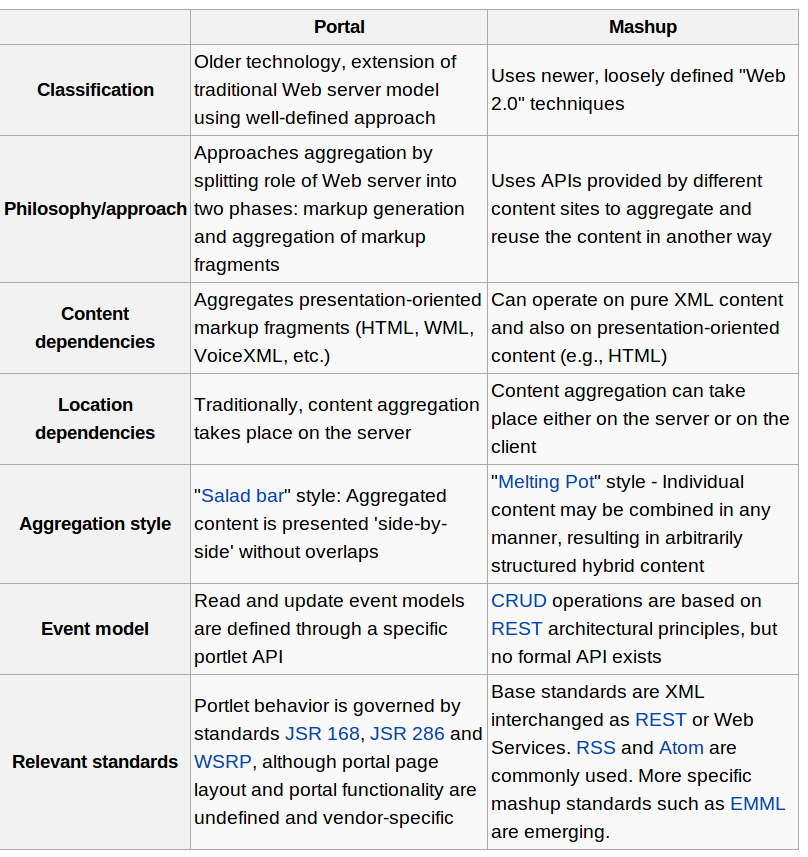
\includegraphics[scale=0.8]{images/MashupVsPortal.png}   
\caption[Comparative Characteristic of Approaches]{Comparative Characteristic}
\label{img:comparative characteristic}                           
\end{figure}
